\section{Vortex Generator}

It is desirable to enhance understanding of 
trailing axial vortices generated by aircraft wingtips and their behavior.
While naturally occurring axial vortexes occur in unpredictable and non-uniform 
environments, this experimental investigation required that a repeatable axial 
vortex.  Small-scale aircraft axial wake vortices can be generated in an 
enclosed wind tunnel environment with a single wingtip, but the downwash 
behavior of a wingtip vortex is distorted by the walls of the wind tunnel and 
test section. A bi-wing vortex generator, as pictured in Figures 
\ref{fig:vortex_gen} and \ref{fig:vortex_design}, was designed and constructed 
by undergraduate student researchers to generate a vortex formed by merging two 
juncture vortices of opposite sign and resulting in a single vortex, absent any 
downwash \cite{davis2012}. The vortex generator employed two symmetric NACA-0012
airfoils with chord length of 101.6$mm$ manufactured from foam casts attached 
to a 25.4$mm$ diameter cylindrical center body with hemispherical forward and 
aft end caps. While the vortex generator could be permitted to have variable
angles-of-attack, the wings were locked at an angle of attack of $\pm$8 degrees 
to avoid vortex structural distortions that could result from non-repeatable 
changes in angle-of-attack.

\begin{figure}[H]
\centering
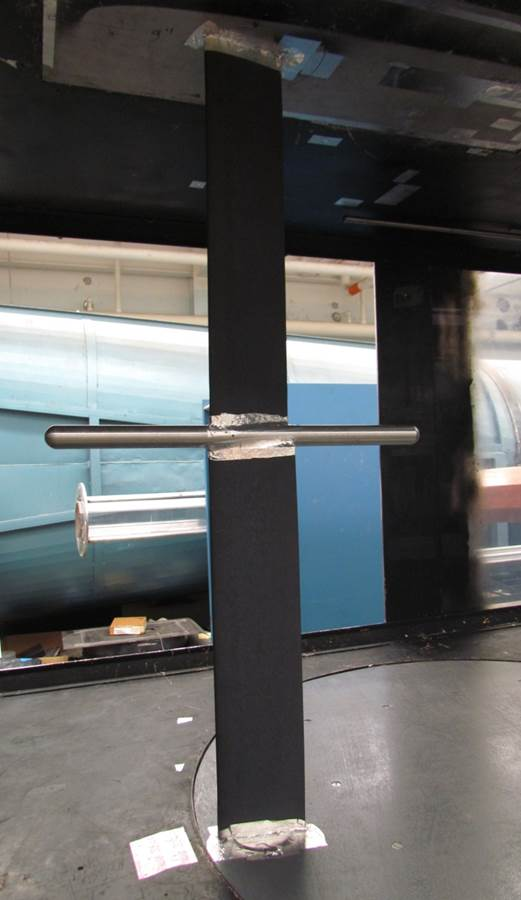
\includegraphics[width=4in]{figs/setup/vortex_generator/picture}
\caption{Picture of the vortex generator set up in the ODU LSWT.}
\label{fig:vortex_gen}
\end{figure}

\begin{figure}[H]
\centering
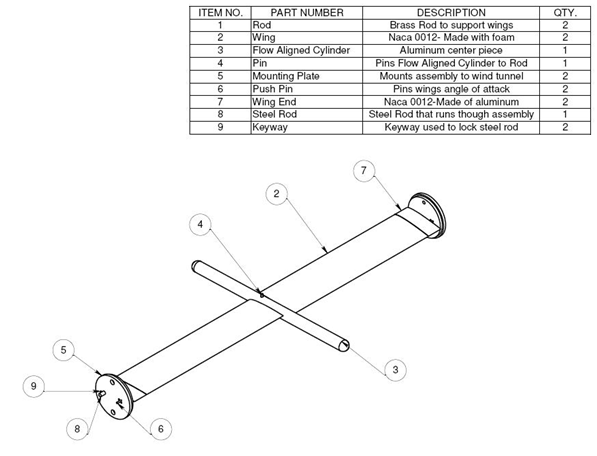
\includegraphics[width=6.5in]{figs/setup/vortex_generator/design}
\caption{CAD design of the vortex generator used in this study.}
\label{fig:vortex_design}
\end{figure}

